
Attenuation refers to a reduction in the strength of a signal.
 Attenuation occurs with any signal, whether digital or analogue. 
Seen the aim of making a network the first step is to look into  
what frequencies can be transmitted and received.
\newline
In the environment in which we want our project to take place, we want the following:
 \begin{enumerate}
	\item An antenna that a high so we can affect the data rate of the signal
	\item A frequency range at which Attenuation is not present 
 \end{enumerate}
Through research, I found the following plots:

\newpage

\begin{enumerate}

	\item  First Plot
	The first plot  I got for Savage e.t al pg. 7 \cite{Savage}
	\begin{figure}[h!]
		\centering
		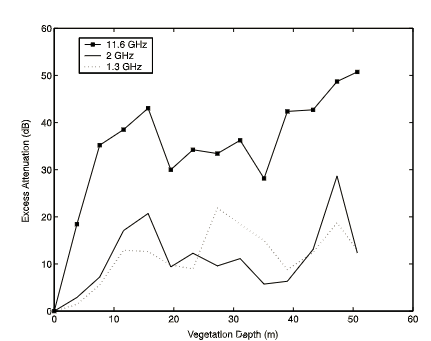
\includegraphics[width=0.5\linewidth]{Images/Silver_Maple.png}
		\caption{Silver Maple in-leaf excess attenuation for the line of trees geometry (receiver antenna height: 3.5 m, SAVAGE ET AL.pg.7}
		\label{Silver Maple in-leaf excess attenuation for the line of trees geometry (receiver antenna height: 3.5 m, SAVAGE ET AL.pg.7}
	\end{figure}
 
This graph displays as vegetation depth increases  Attenuation rises. The problem with this graph is that it doesn't give an in-depth view of which attenuation occurs.
This then led me to look up the International Telecommunication Union  \cite{ITU} recommendations for Attenuation in wooded areas



	\item Second Plot
\begin{figure}[h!]
		\centering
		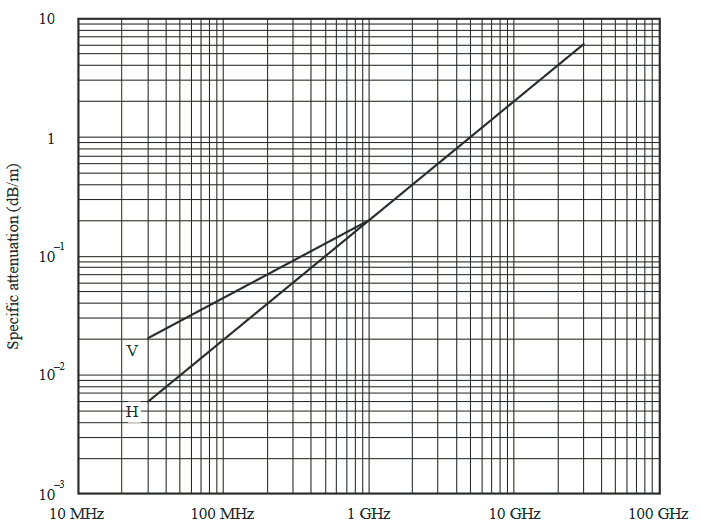
\includegraphics[width=0.5\linewidth]{Images/ITU attteuntion.png}
		\caption{Specific attenuation due to woodland (Recommendation ITU-R P.833-7 (02/2012) Attenuation in vegetation pg.5}
		\label{Specific attenuation due to woodland (Recommendation ITU-R P.833-7 (02/2012) Attenuation in vegetation pg.5}
		\end{figure}
	V is the vertical polarization
	H is the horizontal polarization

	From this graph we  can assume the following:
	\begin{enumerate}
		\item From a frequency $\ge$15GHz we can assume Attenuation is more components
		\item Around the 1 GHz range we  get low values of Attenuation
		\item in the  MHz range we get the best response
	\end{enumerate}
	from this, I selected the  range which is  $10^6 hz$
	
\end{enumerate}
\newpage
so now that  we  established our range let us consider  what happens when it rains

\cite{Sabetahd_Mousavi_Ghasemi_Vafaei_Poursorkhabi_Mohammadzadeh_Zandi_2022}

\begin{figure}[h!]
	\begin{center}
		
	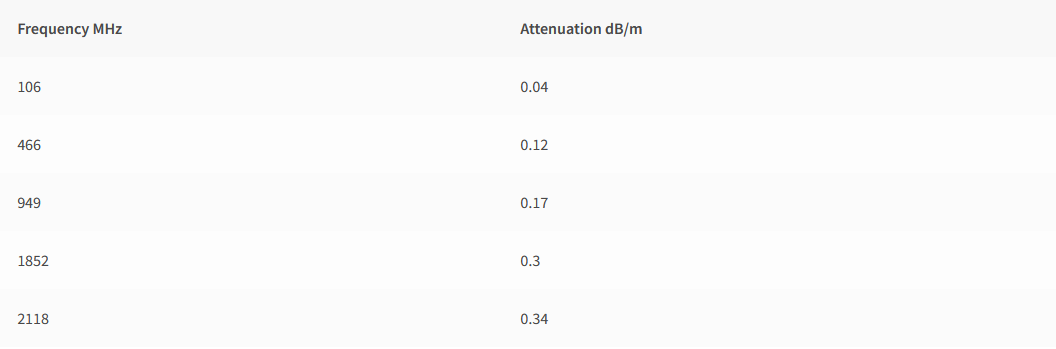
\includegraphics[width=\linewidth]{Images/atteuntion_2.png}\par
	\caption{Predicted attenuation due to rain for the region, which is measured by using the ITU standards,(Source: Hindawi(2014))}
	\label{Predicted attenuation due to rain for the region, which is measured by using the ITU standards,(source: Hindawi(2014))}
		\end{center}
\end{figure}
Ideally, we want a low MHz but we want speed and this  is dictated by what we choose let's further see how radio waves are affected by water/rain
\subsection{Absorption of water}
for this, I found this graph from Lunken Heimer \cite{lunken} 

\begin{figure}[h!]
	\centering
	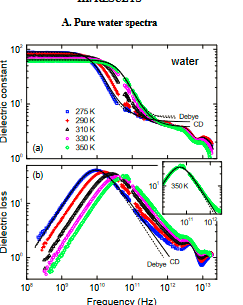
\includegraphics[width=0.5\linewidth]{Images/absorstion.png}
	\caption{absorption of water}
	\label{absorption of water}
\end{figure}

According to the  graph, Water absorbs MHz frequencies which will affect the  transmission 
in the transmission and in some cases, we might have to consider non-line-of-sight communication when it rains or we might also consider another node to route to receive the node.

